% Options for packages loaded elsewhere
\PassOptionsToPackage{unicode}{hyperref}
\PassOptionsToPackage{hyphens}{url}
%
\documentclass[
]{article}
\usepackage{lmodern}
\usepackage{amssymb,amsmath}
\usepackage{ifxetex,ifluatex}
\ifnum 0\ifxetex 1\fi\ifluatex 1\fi=0 % if pdftex
  \usepackage[T1]{fontenc}
  \usepackage[utf8]{inputenc}
  \usepackage{textcomp} % provide euro and other symbols
\else % if luatex or xetex
  \usepackage{unicode-math}
  \defaultfontfeatures{Scale=MatchLowercase}
  \defaultfontfeatures[\rmfamily]{Ligatures=TeX,Scale=1}
\fi
% Use upquote if available, for straight quotes in verbatim environments
\IfFileExists{upquote.sty}{\usepackage{upquote}}{}
\IfFileExists{microtype.sty}{% use microtype if available
  \usepackage[]{microtype}
  \UseMicrotypeSet[protrusion]{basicmath} % disable protrusion for tt fonts
}{}
\makeatletter
\@ifundefined{KOMAClassName}{% if non-KOMA class
  \IfFileExists{parskip.sty}{%
    \usepackage{parskip}
  }{% else
    \setlength{\parindent}{0pt}
    \setlength{\parskip}{6pt plus 2pt minus 1pt}}
}{% if KOMA class
  \KOMAoptions{parskip=half}}
\makeatother
\usepackage{xcolor}
\IfFileExists{xurl.sty}{\usepackage{xurl}}{} % add URL line breaks if available
\IfFileExists{bookmark.sty}{\usepackage{bookmark}}{\usepackage{hyperref}}
\hypersetup{
  hidelinks,
  pdfcreator={LaTeX via pandoc}}
\urlstyle{same} % disable monospaced font for URLs
\usepackage{longtable,booktabs}
% Correct order of tables after \paragraph or \subparagraph
\usepackage{etoolbox}
\makeatletter
\patchcmd\longtable{\par}{\if@noskipsec\mbox{}\fi\par}{}{}
\makeatother
% Allow footnotes in longtable head/foot
\IfFileExists{footnotehyper.sty}{\usepackage{footnotehyper}}{\usepackage{footnote}}
\makesavenoteenv{longtable}
\usepackage{graphicx}
\makeatletter
\def\maxwidth{\ifdim\Gin@nat@width>\linewidth\linewidth\else\Gin@nat@width\fi}
\def\maxheight{\ifdim\Gin@nat@height>\textheight\textheight\else\Gin@nat@height\fi}
\makeatother
% Scale images if necessary, so that they will not overflow the page
% margins by default, and it is still possible to overwrite the defaults
% using explicit options in \includegraphics[width, height, ...]{}
\setkeys{Gin}{width=\maxwidth,height=\maxheight,keepaspectratio}
% Set default figure placement to htbp
\makeatletter
\def\fps@figure{htbp}
\makeatother
\setlength{\emergencystretch}{3em} % prevent overfull lines
\providecommand{\tightlist}{%
  \setlength{\itemsep}{0pt}\setlength{\parskip}{0pt}}
\setcounter{secnumdepth}{-\maxdimen} % remove section numbering

\author{}
\date{}

\begin{document}

\hypertarget{extended-gcc-compiler}{%
\section{Extended GCC Compiler}\label{extended-gcc-compiler}}

The Extended GCC compiler development system is a compiler generator
that automatically creates an executable compiler out of an architecture
description. In our case, ASIP Meister automatically creates this
architecture description itself and an afterwards running program
provided by the developers of ASIP Meister. In this chapter, some basics
about the buildup of retargetable compilers, creation and usage of a GCC
compiler for our specific ASIP Meister CPU's are explained.

\hypertarget{basics-about-retargetable-compilers}{%
\subsection{Basics about Retargetable
Compilers}\label{basics-about-retargetable-compilers}}

Figure~8‑1:
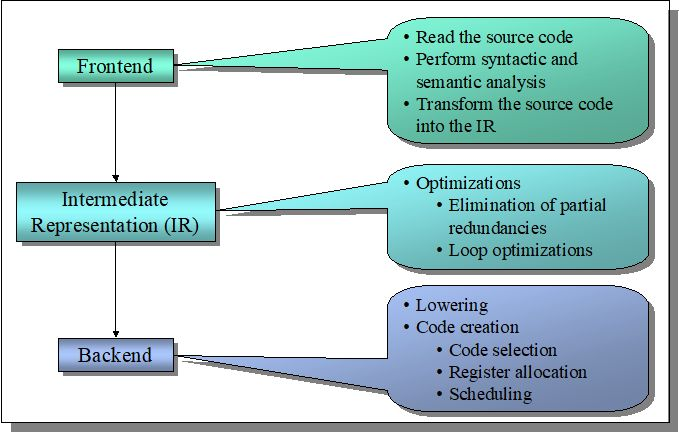
\includegraphics[width=5.52292in,height=3.49444in]{8-1.png}
A Typical Buildup for a Retargetable Compiler

A typical retargetable compiler is separated into \textbf{three} phases,
as shown in Figure~8‑1. The first stage is architecture independent, but
source language dependent. This phase reads the source code, inspects it
for syntactic and semantic correctness, and transforms it into the
second phase, the intermediate representation (IR). This IR is as well
source language independent as architecture independent and it is used
to perform the optimizations. This implies, that the optimizations can
be easily reused, if the source language or the architecture changes.
The third phase is source language independent, but highly architecture
dependent. This backend first transforms the IR into a low-level form.
That means, that high-level structures, like polymorphic procedure calls
are replaced by jump tables or that complex data structures are
disassembled into elementary memory accesses. Afterwards the final
assembly code has to be created. This part is separated into
\textbf{three} steps. In the first step, code has to be selected out of
the lowered IR. This code selection is not unique, as there are always
different possibilities to represent some statements in assembly
language. This code selection works with virtual registers, which are
replaced by real registers in the second step. This register allocation
might lead to additional stack accesses for swapping values out, if no
free real register can be found to hold the value of a virtual register.
In the third step, the code is scheduled, to minimize penalties for data
dependencies. Every step from this code selection has a great influence
on the outcome of the other steps. The sequence of these steps is not
determined and different compilers work with different sequences. The
above given order is just exemplary.

\hypertarget{creating-the-extended-gcc-compiler-in-asipmeister}{%
\subsection{Creating the Extended GCC Compiler in
ASIPmeister}\label{creating-the-extended-gcc-compiler-in-asipmeister}}

The ASIP Meister complier generation supports the base processor
Brownie. In order for the compiler to generate instructions that are
extended from the Brownie processor, some definitions are necessary.
Using {[}C Definitions{]}, you can define the C description
specifications that are supported by the ASIP Meister compiler and the C
description variables that support the instructions extended from the
Brownie processor. The ``Compiler Generation'' is possible only for the
processor extending a base processor Brownie. One can define how to
represent the extension instruction added to the base processor Brownie
in C code during the ``C Definition'' stage. Extension instruction
definition enables a complier to output assembly code complying with the
extension instruction.

\hypertarget{c-definition}{%
\subsubsection{C Definition}\label{c-definition}}

On the ``Ckf Prototype'' tab of ``C Definition'' sub-window in
ASIPmeister, you can define all the newly defined instructions as
described in the Page-65 of {[}TUT{]} and on the Page-57 of {[}UM{]}

\hypertarget{compiler-generation}{%
\subsubsection{Compiler Generation}\label{compiler-generation}}

At ``Compiler Generation'' stage in ASIPmeister, the processor compiler
and the Binutils can be generated. The processes involved in the
``Compiler Generation'' phase are as follows.

1. Input Description Generation: select and run.

2. GNU Tools Generation: select and run.

If you select ``Input Description Generation'' from the drop down list,
the compiler extended description will be generated. After the
generation terminates successfully, if the design data file was called''
browstd32.pdb'', a new directory called'' browstd32.swgen'' will be
generated inside ''meister'' directory, and inside this directory the
compiler extended description is generated in a file named ''
browstd32.xml''. The generated compiler and Binutils supports the Ckf
defined at ``C Definition''. After you select ``GNU Tools Generation''
and the generation terminates successfully, the compiler and the
Binutils will be generated in default directory called
''browstd32.swgen'' in the ``meister'' directory.

\hypertarget{using-custom-instruction-in-the-c-program}{%
\subsubsection{Using custom instruction in the C
Program}\label{using-custom-instruction-in-the-c-program}}

Once the custom instruction is defined in the ``C Definition'', they can
be used in the C program as described on the Page-63 in {[}UM{]} and on
Page-68 in {[}TUT{]}. There are two methods to use the custom
instruction here:

\begin{enumerate}
\def\labelenumi{\arabic{enumi}.}
\item
  When you want to write the extended instruction description in C code,
  you have to add ``\_\_builtin\_brownie32\_'' directive to the ``ckf
  definition''. An example is demonstrated in the following for a custom
  instruction AVG with three parameters (AGV rd, rs1, rs2).
\end{enumerate}

int a=12,b=23,c;

c = \_\_builtin\_brownie32\_AVG(a, b);

\begin{enumerate}
\def\labelenumi{\arabic{enumi}.}
\setcounter{enumi}{1}
\item
  In some cases, above method does not work, e.g., when an instruction
  returns a ``void''. Standard inline assembly directives can be used to
  write the extended custom instruction, as follows:
\end{enumerate}

\_\_asm\_\_ volatile (

"avg \%{[}my\_out{]}, \%{[}my\_op1{]}, \%{[}my\_op2{]}\textbackslash n"

: {[}my\_out{]} "=\&r" (c)

: {[}my\_op1{]} "r" (a),{[}my\_op2{]} "r" (b)

);

\hypertarget{using-the-extended-gcc-compiler}{%
\subsubsection{Using the Extended GCC
Compiler}\label{using-the-extended-gcc-compiler}}

In the lab, the Makefile is automatically doing all the steps. However,
you can also use the generated compiler separately; the following
demonstrates a method for cross compiling a C program file called
``bubble.c''.

\begin{enumerate}
\def\labelenumi{\arabic{enumi}.}
\item
  First, you have to add the path ``browstd32.swgen/bin'' to the \$PATH
  environment variable.
\end{enumerate}

export COMPILER\_DIR=/brownie/meister/browstd32.swgen/bin

or

export PATH=/brownie/meister/browstd32.swgen/bin:\$PATH

\begin{enumerate}
\def\labelenumi{\arabic{enumi}.}
\setcounter{enumi}{1}
\item
  Compile the C program into .s assembly file
\end{enumerate}

\$\{COMPILER\_DIR\}/brownie32-elf-gcc -S -combine -O3 bubble.c -o
bubble.s

\begin{enumerate}
\def\labelenumi{\arabic{enumi}.}
\setcounter{enumi}{2}
\item
  Assemble bubble.s file into .o object file. Also, assemble startup.s
  (startup code) and handler.s (interrupt handler) file to object files.
\end{enumerate}

\$\{COMPILER\_DIR\}/brownie32-elf-as -o startup.o startup.s;

\$\{COMPILER\_DIR\}/brownie32-elf-as -o handler.o handler.s;

\$\{COMPILER\_DIR\}/brownie32-elf-as -o bubble.o bubble.s;

\begin{enumerate}
\def\labelenumi{\arabic{enumi}.}
\setcounter{enumi}{3}
\item
  Link the object files using the linker script ``browtb.x''. This
  script declares some important information about the stack pointer,
  text and data sections, program counter address after the resetting
  the CPU.
\end{enumerate}

\$\{COMPILER\_DIR\}/brownie32-elf-ld -o bubble -T browtb.x
bubble\_uart.o startup.o handler.o

\begin{enumerate}
\def\labelenumi{\arabic{enumi}.}
\setcounter{enumi}{4}
\item
  Converting compiled object file to memory image of the C program. Use
  ``gccout2img'' for a file in elf format obtained through normal
  compilation. The script ``gccout2img'' outputs \emph{TestData.IM} and
  \emph{TestData.DM}, with which the user can perform simplified test
  simulations.
\end{enumerate}

gccout2img bubble

\hypertarget{library-with-standard-functions-for-asip-meister-gcc-hardware-prototype}{%
\subsection{Library with Standard Functions for ASIP Meister / GCC /
Hardware
Prototype}\label{library-with-standard-functions-for-asip-meister-gcc-hardware-prototype}}

Many applications use some standard library calls like \emph{printf},
\emph{malloc} or \emph{atoi} that are not declared in the standard of
the C programming language, but which are nevertheless declared in the C
standard library. Now, GCC is a compiler for the C language and does not
provide an implementation for the standard library (in fact there are
some huge fragments that would have to be adapted to our specific
environment, what has not been done due to the complexity of a full
run-time implementation).

To close the gap between a plain C compiler and the wish of letting
complex algorithms run in hardware and produce understandable output we
are providing some basic \emph{stdlib} functionality, which is dedicated
to the environment of ASIP Meister, the GCC compiler and our hardware
prototype. This basic \emph{stdlib} functionality is extended on demand
to reflect the latest changes of our environment. Thus, it is not
explained exhaustively or in high detail. Instead, the underlying
concepts and the needed steps for using the basic \emph{stdlib} library
is explained here, plus some of the main functions for using our touch
screen LCD with some examples.

All typical functionalities of our \emph{stdlib} implementation are
available in the directory \emph{/home/asip00/epp/StdLib/.} The
functionality is encapsulated into a header file that is providing the
interface and a documentation of the functionality and a C file for
implementing the header. You can use these files by linking/copying them
into your application project subdirectory and using ``\emph{make sim}''
to compile your application and the \emph{stdlib} files into one binary
and simulation file, as it will be shown in the example below. Linking
to the files instead of copying them has the advantage, that you always
have the latest version of these files in your project. Some of the
files in the \emph{stdlib} directory have dependencies to other files of
this directory. Thus, you can get a compiler error, that a specific
header file was not found when you try to compile your project. You then
have to manually link to the dependent files as well. Just linking to
all available files is generally not a good idea, as this makes the
compilation process take longer and it increases the needed memory size
of your application.

Now we will demonstrate how you can create a small application that is
using the LCD of the hardware prototype:

\begin{itemize}
\item
  Create a new subdirectory inside the application directory of your
  ASIP Meister project and change into this new directory
\item
  Copy or Link to \emph{lib\_lcd}, \emph{loadStorByte} and
  \emph{string}, by executing:
\end{itemize}

\begin{quote}
ln --s /home/asip00/epp/StdLib/lib\_lcd\_320.* .

ln --s /home/asip00/epp/StdLib/loadStoreByte.* .

ln --s /home/asip00/epp/StdLib/string.* .

\emph{lib\_lcd} has a dependency to \emph{loadStoreByte} and
\emph{string}, that is why you need both.

The \emph{lib\_lcd\_320} exists in different C implementations,
depending on your target LCD. One C file is for the LCD with a 240x128
resolution, the other one is for the 320x240 resolution, and the last
one is for the dlxsim simulation. Make sure that at most, one of these C
files is available in your application subdirectory; otherwise, the
linker will complain about multiple implementations (one per C file) of
the LCD functionality.
\end{quote}

\begin{itemize}
\item
  Prepare an ``\emph{env\_settings}'' file, as shown in Chapter~6.4.
\item
  Add a new C file that contains your main method. This main method will
  contain the following code as example:
\end{itemize}

\begin{quote}
t\_print(``Hello World\textbackslash r\textbackslash n'');

t\_printInt(42);

The LCD needs the ``\emph{\textbackslash r\textbackslash n}'' in the
string, as it is handling carriage return (\textbackslash r) and line
feed (\textbackslash n) independently.
\end{quote}

\begin{itemize}
\item
  Compile your project by executing ``\emph{make sim}''.
\end{itemize}

The resulting program can be simulated with dlxsim or ModelSim or it can
be uploaded to the hardware prototype (explained in Chapter~6.4)
depending on the selected LCD library.

After you have once compiled a C-Code that rarely changes (e.g. the
libraries), you can reuse the created assembly code for future
compilations. That will enormously speed up the whole compilation
process. This is especially good for all applications in the
\emph{StdLib} directory. Just compile them one time with ``\emph{make
sim}'' and then copy the created .\emph{asm} file from the
``\emph{BUILD\_SIM}'' directory to the directory of your other
application files, but name it .s instead of .asm. Then remove the C
code (but not the header) to make sure the code does not exist twice (in
the C code and in the Assembly file). For instance:

cp BUILD\_SIM/loadStoreByte.asm loadStoreByte.s

rm loadStoreByte.c

However, when moving from dlxsim to FPGA implementation then you have to
delete these assembly files, link to the C files, and recompile them. If
you are often switching between dlxsim and FPGA, then it may be
beneficial to create two application directories with the different
libraries and ``\emph{env\_settings}'' specified for dlxsim and FPGA
respectively and using the same application-specific source code in both
directories (e.g. with a link).

As mentioned above, the ``\emph{lib\_lcd}'' exists in different
variants. The files ``\emph{lib\_lcd\_240.c}'' and
``\emph{lib\_lcd\_320.c}'' are for the FPGA prototype. They implement
the real protocol for communicating with the I\textsuperscript{2}C bus
and thus with the LCD. For a simulation, we cannot use this
implementation, as it is waiting for certain responses from
I\textsuperscript{2}C/LCD, but in dlxsim/ModelSim simulation, these
answers will never appear. We have therefore implemented
``\emph{lib\_lcd\_­dlxsim.c}'' which simply writes every single
character that is send to the LCD to an output file (a virtual LCD).
This is a very good debugging possibility for printing text, although it
is not helpful for any graphic output to the LCD (e.g. lines, bars
\ldots), as these control words are hard to understand manually. For
dlxsim, the characters are either printed to the console whenever they
appear or they are collected and printed to a file (parameter ``-lf'' in
Chapter~3.2.1). For ModelSim, the characters are printed to a file
``\emph{lcd.out}'' in the ModelSim directory. The header file
``\emph{lib\_lcd.h}'' is valid for all C files, but you have to make
sure, that at most one of the both C files is available in the directory
when compiling with ``\emph{make sim}''. Otherwise, you will get two
implementations of the LCD functions and the assembler will complain,
that he cannot decide which one to choose.

\hypertarget{functions-of-the-lcd-library}{%
\subsubsection{Functions of the LCD
Library}\label{functions-of-the-lcd-library}}

This chapter summarizes some of the available functions to access the
features of the LCD of our hardware prototyping board. The library also
contains some high-level functionality that is useful, but introduces a
dependency to ``\emph{string.c}''. Therefore, this library has to be
provided as well when using ``\emph{lib\_lcd}''.

The most important basic I/O instructions are:
``\emph{t\_print(char*)''}, ``\emph{t\_printInt(int)''}, and
``\emph{t\_printHex(int value, int digits)''}. You can use them to print
strings and numbers, for instance:

char tempString{[}{]} =
``\textbackslash r\textbackslash n\textbackslash t\textbackslash t'';

t\_print(``Hello World!'');

t\_print(tempString);

t\_printInt(23);

t\_print(`` = ``);

t\_printHex(23, 0);

t\_print(tempString)

t\_printInt(42);

t\_print(`` = ``);

t\_printHex(42, 4);

The ``\emph{printHex()''} function can trim the output to a given number
of digits (4 in this case). To not trim the number of digits you have to
give `0' as parameter. The output of the above example looks like:

Hello World!

23 = 0x17

42 = 0x002A

In the following, we describe further functions of the LCD. Some of them
are generally sending a command to the LCD (you have to use the LCD
manual {[}eDIP{]} to find the available commands) and some of them are
offering typical commands (e.g. \emph{drawline}) as convenience
functions.

int checkbuffer()

This function returns the number of available bytes in the send buffer
of the LCD. It can be used to wait for a return value of the LCD. For
example when pressing a button on the touch panel, a value of this
button is written to the LCD send buffer.

int getbytes (char* dest, int bytes\_to\_read)

This reads a specific number of bytes from the send buffer. With the
``\emph{checkbuffer''} function, you can test how many bytes are
available in the buffer.

int sendcommand ( const char cmd0, const char cmd1,
const~int~options{[}{]}, const char text{[}{]},\\
int intcount, int charcount, int address)

This is a general function for sending commands to the LCD. The
following commands internally use ``\emph{sendcommand''} to realize
their functionality. The parameters of ``\emph{sendcommand''} are:

\begin{itemize}
\item
  Two chars, specifying the command
\item
  Depending on the type of the command, some options
\item
  Depending on the type of the command a string with a predefined size
\item
  The address of the LCD (defined in \emph{lib\_lcd.c})
\end{itemize}

int t\_print (const char* str)

This function writes a string to the LCD terminal. The ``\emph{t\_}''
indicates a command for the console mode of the LCD, compared to the
graphic mode (\emph{g\_}) of the LCD, which is explained later.

int t\_cursor (int onoff)

Turns on (1) or off (0) the blinking cursor of the terminal.

int t\_enable (int onoff)

Turns the display on (1) or off (0). When the display is turned off, all
submitted data is ignored. Previously sent data (when the display was
on) is buffered and will become visible again, after the display will
become turned on again.

int g\_print (const char* str, int x, int y)

Writes a string to the coordinates (x, y). You must not send control
signals like \textbackslash n in this function. They are only available
for the t\_print function.

int g\_drawrect (int x1, int y1, int x2, int y2)

int g\_drawline (int x1, int y1, int x2, int y2)

Draws a rectangle/line.

int g\_makebar ( int x1, int y1, int x2, int y2, int low\_val, int
high\_val, int init\_val, int type, int fill\_type, int touch)

Creates a bar graph at the defined coordinates. ``\emph{low\_val''} and
``\emph{high\_val''} describe the minimal and maximal (at most 254)
value of the bar graph. ``\emph{init\_val''} defines the initial value
and ``\emph{type''} and ``\emph{fill\_type''} adjust the appearance of
the graph. Type=1 will draw a bar in a box and the ``\emph{fill\_type}''
(in the range of 1 to 15) then defines the fill pattern. Type=3 will
draw a line in a box and the ``\emph{fill\_type}'' will then define the
thickness of the line. For more details refer too {[}LCD{]}.

With ``\emph{touch''} you can define, whether the bar graph will be user
changeable by the touch screen. Every bar graph gets a unique number,
which is returned by the function. At most 32 bar graphs are supported
by the display. When the touch screen functionality is activated and the
user changes the value of the bar graph, the LCD automatically writes
the number of the changed bar graph and its modified value to the
buffer, from where it can be received with the checkbuffer and getbytes
function.

int g\_setbar (int barnum, int value)

Sets an existing bar graph to a specific value.

int g\_makeswitch ( const char* str, int x1, int y1, int x2, int y2, int
down, int up)

Creates a switch (button) with a label. The parameter ``\emph{str''}
contains this label, preceded by a control char which defines the
alignment of the label. ``C'' means centered, ``L'' means left- and
``R'' means right-aligned. \emph{down} and \emph{up} define the code,
which the LCD will write into the send buffer, when the button is
pressed or released. When 0 is provided as parameter for up or down,
then nothing will be written to the buffer for the specific activity.

int g\_makeradiogroup (int group\_number)

A new defined switch can be assigned to a specific radio group. A radio
group automatically makes sure, that at most one switch of the group is
pressed.

int g\_makemenubutton ( const char* str, int x1, int y1, int x2, int y2,
int down, int up, int select, int space)

A menu item is created. With ``\emph{str''} you can define the
appearance and the menu entries. The first character defines the
direction in which the menu will open (``L'': left, ``R'': right, ``O''
up, ``u'': down). The second char defines the alignment of label on the
menu item (``C'': centered, ``L'': left aligned, ``R'': right aligned).
The labels of the menu entries follow afterwards and are separated by a
``\textbar'' sign. ``\emph{down''} defines the value that will be
written to the buffer, when the menu item is pressed and up defines the
value that will be written to the buffer, when the menu is closed,
without choosing a specific entry (aborted). ``\emph{select''} defines
the base value that is used to compute the value that will be written to
the LCD buffer, when a menu entry is chosen. This value is computed as:
base value~+~entry number~--~1. ``s\emph{pace''} defines the gap in
pixels between the menu entries. This is a global value, thus it will
also change the appearance of already existing menus.

\hypertarget{functions-of-further-libraries}{%
\subsubsection{Functions of Further
Libraries}\label{functions-of-further-libraries}}

Besides the LCD, further functionality and helping functions are
available. They will be summarizes in this section to give an overview
of the available features. You should look into the libraries to find
out more.

\textbf{lib\_uart:} besides printing to LCD, you may also print to the
UART port using the ``\emph{u\_print''}, ``\emph{u\_printInt''}, and
``\emph{u\_printHex''} functions (similar to ``\emph{t\_print''} etc.).
You can read from the UART port with ``\emph{u\_getbytes''}. However,
you need a HyperTerminal running at the pc to which the UART is
connected (see Chapter~6.4.2 for details about the HyperTerminal). In
Modelsim, uart.out is automatically created while for dlxsim you can
pass the parameter ``-uf'' to print text in a file instead of appearing
on the console.

\textbf{lib\_audio:} you can write uncompressed PCM audio data to an
audio port using the ``\emph{audioAddressR\{L\textbar R\}}'' pointers.
The corresponding sample width of the corresponding IP core in the
VHDL-framework (default 16 Bit) can be configured in
``\emph{AudioOut\_Types.vhd''} and the sampling rate (default 40 KHz)
can be configured in ``\emph{dlx\_Toplevel.vhd''} (search for
`i\_audio\_out').

\textbf{lib\_clock:} you can use the pointer ``\emph{clockAddress}'' to
read and write to access a special register that automatically
increments by one in each cycle. You can use this to benchmark the
performance of a certain C-Code by e.g. writing a `0' to it to start the
benchmark and to read it again at the end of the benchmark. Make sure
that the code that will be benchmarked does not contain any unnecessary
I/O instructions (e.g. ``\emph{t\_print''}) as they are extremely slow.

\textbf{String:} contains some typical string manipulation functions,
e.g. ``\emph{strlen''}, ``\emph{strcat''}, ``\emph{strcpy''} \ldots{} It
additionally contains two functions to convert an integer number to a
string representation, as it is used in the I/O libraries, e.g.
``\emph{t\_printInt''} or ``\emph{u\_printHex''}.

\hypertarget{changing-the-frequency}{%
\subsubsection{\texorpdfstring{Changing the Frequency
}{Changing the Frequency }}\label{changing-the-frequency}}

In order to change the frequency of your design and see if it still
works or not (required for the last Session), the Framework contains a
DCM (Digital Clock Manager) that generates five different clocks. By
changing the knob on the external PCB, a multiplexer (in the
``dlx\_toplevel.vdh'' file) selects the corresponding frequency that you
want to apply on your design.

\begin{longtable}[]{@{}ll@{}}
\toprule
Knop value & Frequency (MHz)\tabularnewline
\midrule
\endhead
0 & 100\tabularnewline
1 & 80\tabularnewline
2 & 66\tabularnewline
3 & 50\tabularnewline
4 & 40\tabularnewline
5 & 25\tabularnewline
Else & 100\tabularnewline
\bottomrule
\end{longtable}

Figure 8‑1: Knob Position \& Corresponding Frequencies

\end{document}
